\title{Spectral Analysis and Signal Processing}
\author{
        Kevin Belleville \\
        University of California, Los Angeles\\
        Physics 188B, Josh Samani\\
}
\date{\today}

\documentclass[12pt]{article}

\usepackage{braket}
\usepackage[margin=1in]{geometry}
\usepackage{graphicx}
\usepackage{float}

\begin{document}
\maketitle

\begin{abstract}
By performing Fourier analysis on the monthly mean sunspot numbers and the cosmic ray counts, we learn how to use the Fast Fourier Transform and how to normalize it to analyze real world data.
\end{abstract}

\section*{Introduction}

Although I know these following sections are basically restating what is said in the project description, it is useful for me to retype it. It helps me understand what is happening, when I can begin to explain it myself.

\subsection*{Fourier Transform}

The Fourier transform is a very useful tool in mathematics and physics that allow us to analyze data in useful ways. A common metaphor is that the Fourier transform can "discover" the ingredients of a smoothie, or recreate the smoothie from its ingredients with the inverse. Some common applications are decomposing a signal, filtering out unwanted frequencies, then recreating the cleaner, or easier to manage signal. Mathematically, the fourier transform is defined as:

\begin{equation}
\hat{X}_k = \frac{1}{T} \int^{T}_{0} X(t) \exp{\left( -2\pi i kt/T \right)} d t
\end{equation}

\begin{equation}
X(t) = \sum_{k=-\infty}^{\infty} \hat{X}_k \exp{\left( 2\pi i kt/T \right)}
\end{equation}

Here, a periodic function can be mapped to the sum of its sinusoidal waves $X(t)$, whose coefficients $\hat{X}_k$ define the amplitude and phase of a wave, with its frequency $f(k) = k/T$. However, in the real world, we don't have infinitely long data sets; thus, we use a discrete Fourier transform.

\begin{equation}
\hat{X}_k = \sum_{n=0}^{N-1} X_n \exp{\left( -2 \pi i k n / N \right)}
\end{equation}

\begin{equation}
X_n = \frac{1}{N} \sum_{k=0}^{N-1} \hat{X}_k \exp{\left( 2 \pi i k n / N \right)}
\end{equation}

where $k = n = 0, 1, 2, ... , N-1$. We can then map $k$ to the correct frequency by using these. If $0 \leq k \leq N/2$:

\begin{equation}
f(k) = \frac{1}{T} k 
\end{equation}

And if $ N/2 < k < N$:

\begin{equation}
f(k) = \frac{1}{T} (k - N)
\end{equation}




\subsection*{Fast Fourier Transform}

In our modern world, we can use computers to do these calculation quickly and efficiently for us. Computing the discrete version of the Fourier transform explicitly as it is stated generates a function that is of complexity $O(n^2)$. However, better algorithms have been invented by very smart people, which allow us to compute the transform in $O(n \log{n})$. This is a massive improvement, seeing how many of the data sets Fourier transforms are used on have thousands if not millions of data points. These algorithms are called Fast Fourier Transform (FFT). The most popular of these is the Cooley-Tukey algorithm. The algorithm breaks down a discrete Fourier transform into many smaller DFTs. A deeper analysis of this algorithm and others like it are for another day, but it is good to understand the basic idea of why this works. The numpy FFT package uses this implentation, which we will be learning to use.




\subsection*{Correlation Functions}

We can also use the Fourier transform to create a correlation function for the signals $X(t)$ and $Y(t)$:

\begin{equation}
C_{X,Y}(\tau) = \lim_{T \longrightarrow \infty} \frac{1}{T} \int_0^T X(t+\tau)Y(t)^* dt
\end{equation}

This correlation function tells us the shift between the two functions, when moved by a time lag $\tau$. If we use the same function for both $X(t)$ and $Y(t)$ is a the autocorrelation function. Of course, this is an integral to infinity, which a computer cannot compute; thus we must convert this into a discrete form. This requires us to pad the $X$ and $Y$ function with zeros, such that:

\begin{equation}
\widetilde{X}_n = X_0, X_1, ..., X_{N-1}, 0, 0, ... 0
\end{equation}

\begin{equation}
\widetilde{Y}_n = Y_0, Y_1, ..., Y_{N-1}, 0, 0, ... 0
\end{equation}

where the arrays are of size $2N$. The correlation function then becomes:

\begin{equation}
C_{X,Y} (l) = \frac{1}{N-|l|} \sum_{n=0}^{2N-1} \widetilde{X}_{n+l} \widetilde{Y}^*_n
\end{equation}

We can rewrite this using the Fourier transforms from before:

\begin{equation}
C_{X,Y} (l(n)) = \frac{1}{N-|l(n)|} \mathcal{F}^{-1} \lbrace \mathcal{F} \lbrace \widetilde{X}_n \rbrace_k \mathcal{F} \lbrace \widetilde{Y}^*_n \rbrace_k \rbrace_n
\end{equation}

The lag function $l$ for $0 \leq n \leq N$ is $l(n) = n$; for $N < n < 2N$, it is $l(n) = n-2N$. This essentially maps all of the positive lag values to the lower half (negative time lags), and the negative to the upper half of the array. 






\section*{Assignment}

\subsection*{Power Spectra}

% Compute power spectra of the signals (sunspots, rays) and estimate the time period (inverse freq)
% of the dominant nonzero frequency mode in the spectrum. The dominant mode should lie in the 
% low-freq range

We can find the power spectrum of a distribution of a wave amplitude by using this equation:

\begin{equation}
P_k = \frac{T^2}{N^2} |X(k)|^2
\end{equation}

This is useful because allows us to remove random, white noise from the signal, focusing on the important data. Below are graphs of the power spectra of both the sunspots and the cosmic rays. It should be noted that these graphs are not of the entire power spectrum, but a zoomed in version on the part of the spectrum we are focusing on -- the first non-zero maximum.

\begin{figure}[H]
\begin{center}
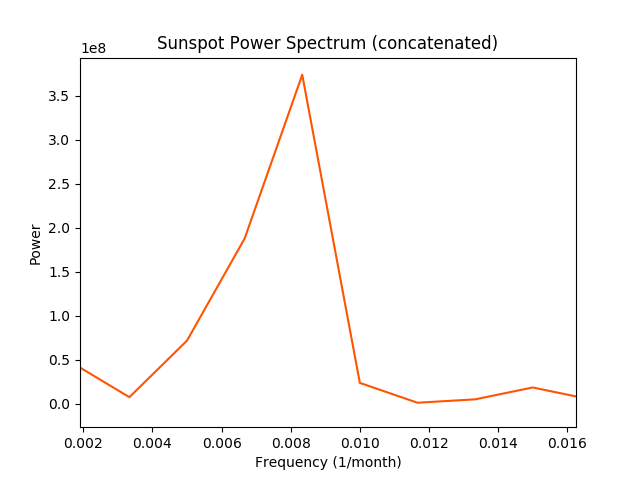
\includegraphics[scale=0.8]{psd_ss.png}
\end{center}
\end{figure}


\begin{figure}[H]
\begin{center}
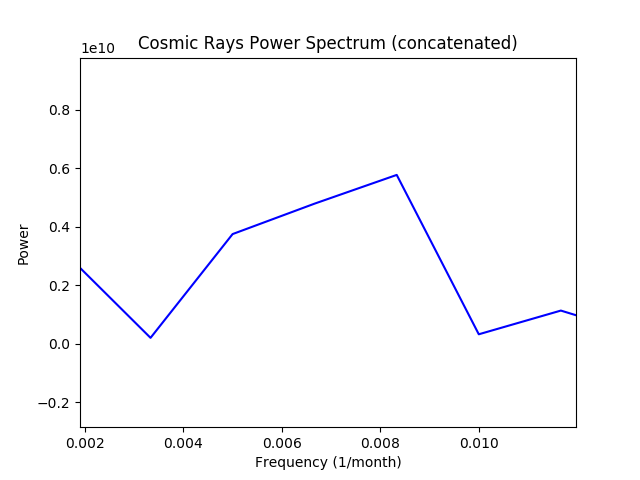
\includegraphics[scale=0.8]{psd_rays.png}
\end{center}
\end{figure}

There is a large spike at zero which is a consequence of the discreteness of the algorithm we use. In the next parts of this assignment we will implement zero padding to make our data easier to use. We couldn't implement it here, as it would change our outcome. Nevertheless, I could see the both of these graphs' global non-zero maximum was at $f=0.00835$ months$^{-1}$. Inverting this to find the time period of the data, we get $T = 9.98$ months. Although the accepted value is about $T=11$ months, this is in the ballpark, and shows that this method is good for estimating the correct value.




\subsection*{Solar and Cosmic Ray Cycles}

% explain equation 11 and 13
% padding the arrays with zeros
% Estimate the length of the solar cycle and the cosmic ray cycle from the time periods of 
% their autocorrelation functions

We can use the correlation function from the introduction to perform autocorrelation by using the same data for both the $X$ and $Y$ components. Before we do this, however, we must utilize zero padding, which is simply doubling the size of the data, and filling the latter half with zeros. This helps the FFT because it allows the FFT to be longer, and produce a longer result. This means that it has more frequency "bins", which is essentially a method of interpolating a large number of points. In our case, specifically, when using the correlation function, it gives the correlation function space for a longer result.

Before we do that, we must normalize the function as well. This is easily done with the relation:

\begin{equation}
A_n \longrightarrow \frac{( A_n - \bar{A} )}{\sigma_A} 
\end{equation}

where $A$ is the function, $A_n$ is a single point in the data, $\bar{A}$ is the time average of $A_n$ and $\sigma_A$ is the standard deviation of $A_n$. 

When I first attempted my own implentation, I ended up with an array of arrays, with correlation functions that had different lags, for all the different values of lag. This led me to an interesting graph, and a small discursion from the regularly scheduled programming, that I'd like to share.

\begin{figure}[H]
\begin{center}
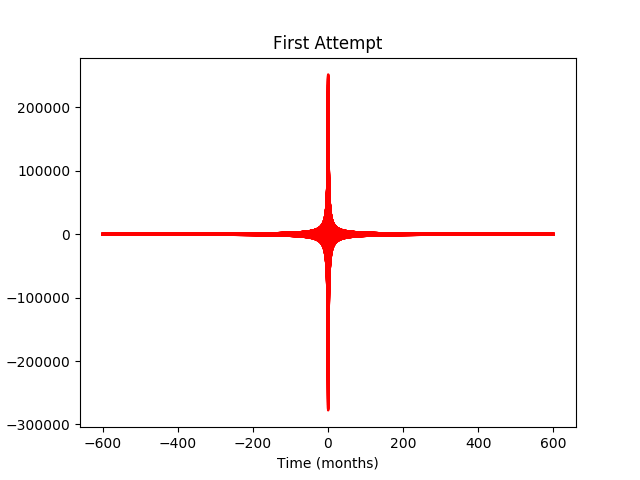
\includegraphics[scale=0.8]{first.png}
\end{center}
\end{figure}

This was weird. I didn't exactly understand what was happening, or why -- but I also had never seen what a correlation function should look like, so I had to do research online. It turns out that this is every different correlation function for each different lag value graphed together. The lag value is the only thing that differentiates one correlation values from the next (in autocorrelation), so I graphed some specific values for lag to show that these are all graphed together, below.


\begin{figure}[H]
\begin{center}
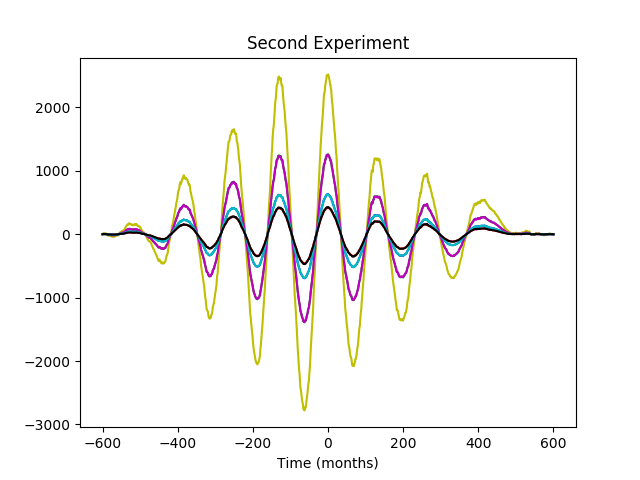
\includegraphics[scale=0.8]{second.png}
\end{center}
\end{figure}

Here we can see that there are multiple graphs plotted together, depending on the lag value. The larger graphs are ones closer to the value of $l=600$, which of course, doesn't exist because we cannot divide by zero. Although this little research doesn't really affect what I am learning today, it was still interesting. Because all of these graphs have peaks and trophs at the same time values, just with different values, they all have the same period, which is what we are looking for in this assignment. So, I simply opened up only one of the graphs to find the period.

\begin{figure}[H]
\begin{center}
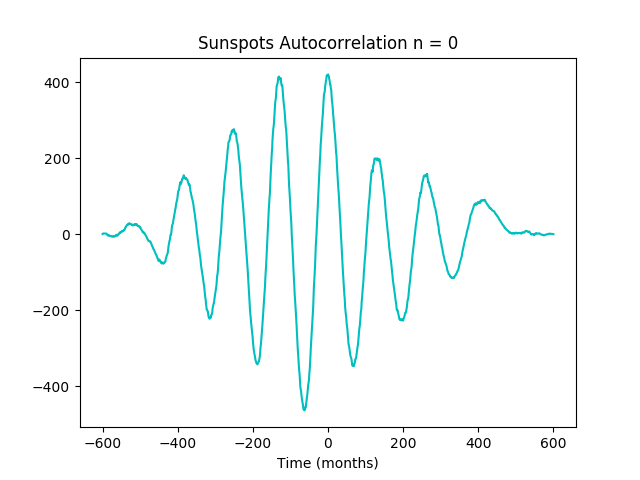
\includegraphics[scale=0.8]{ss_ac.png}
\end{center}
\end{figure}

Although it doesn't make much sense to have a negative time in our data set, this is because of the correlation we are performing. We can still find a period, which I did by cutting the graph in half, to only show the positive values, and finding the first non-zero peak. I ended up with a period of $T=128$ months, which converted into years is $T \approx 10.66$ years. I would also like to say that I attempted to use the numpy function "correlate" which computes the correlation between two signals. From this method, I also achieved the same period of $T=128$ months, which proved to me that my method was accurate enough to use for the rays data as well.


We can do the same for the rays data. For that data we get about $T=10.83$ years. However, it should also be noted that the cosmic ray data was not as sinusoidal as the sunspot data. Below is a graph:

\begin{figure}[H]
\begin{center}
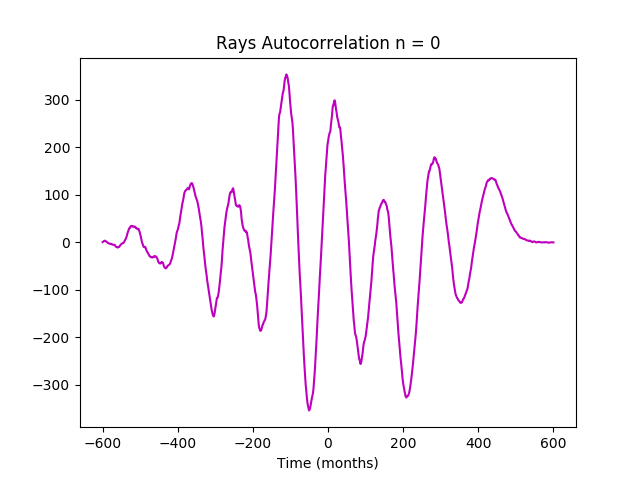
\includegraphics[scale=0.8]{rays_ac.png}
\end{center}
\end{figure}

To find the period of this data, I had to measure from peak to peak.


\subsection*{Normalized Cross-Correlation Function}

% compute the normalized cross-correlation function between the sunspot numbers and the cosmic ray flux
% What is the value of the correlation coefficient C_x,y (l=0)?
% where is the global minimum of the cross-correlation function
% is it exactly at l=0 or is it perhaps slightly shifted

Now, we compute the cross-correlation function between the sunspots data set and the cosmic rays data set. Below is a plot of the cross-correlation:

\begin{figure}[H]
\begin{center}
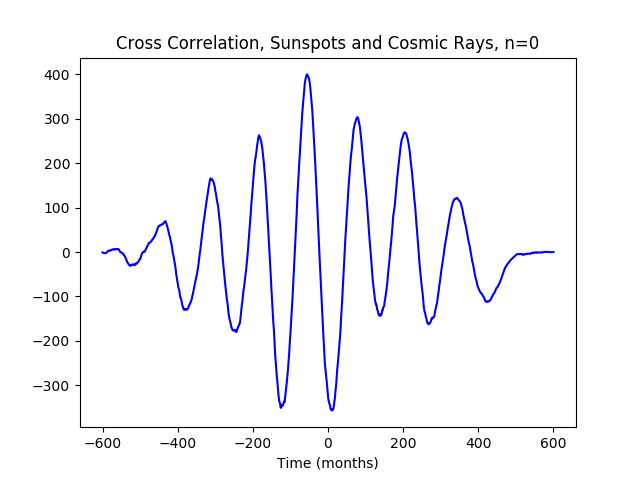
\includegraphics[scale=0.8]{cross.png}
\end{center}
\end{figure}

The value of the correlation coefficient at $l=0$ on my graph is around $-323$. However, it should be noted that correlation coefficients should be between $-1$ and $1$. Although I think I followed the instructions clearly, my plots did not end up that way. Nevertheless, it is quite simple to map the values I received (from its max and min) to values between $-1$ and $1$. After doing so, we see that the correlation coefficient is around $-0.90$ which is very anti-correlated. This makes sense because we know that the sunspot and rays data is anti-correlated.

We also look for the global minimum, which is not at $l=0$, but around $l=10$. This is only very slightly shifted.


It is also interesting, yet maybe redundant, to note that the period of this cross-correlated is also around $T=128$ months, the same as the sunspot period. 



\subsection*{Signal Processing}

% data is noisy
% smooth signals using a SHARP LOW-PASS FILTER with a cutoff freq f_0
% transform the original signal to frequency space, set all modes with frequency |f| >= f_0 to zero
% transform the modified signal back to the time domain
% compare the signals filtered with different cutoff freqs on the same graph

Our data is rather noisy, however, a useful function of the Fourier transform is the ability to manipulate the data before returning it to its time-dependent state. This allows us to filter our certain frequencies. In our case, we will be using a low-pass filter, but there are many different kinds that exist. A low-pass filter basically filters out anything above a certain cutoff frequency. This is useful for us because there may be high frequency that doesn't contribute anything to our data -- rather harms it instead. We can remove this, and still retain the core part of the data that actually matters.

The method for a filter is simple. Given a time-dependent data set, perform a FFT on it to transform it into a frequency-dependent state. Then, for every point, if it is below a certain cutoff freqeuency, leave it be; otherwise, change it to zero. Then perform an inverse FFT to return it to a time-dependent state.

Below is a graph overlaying different cutoff frequencies:

\begin{figure}[H]
\begin{center}
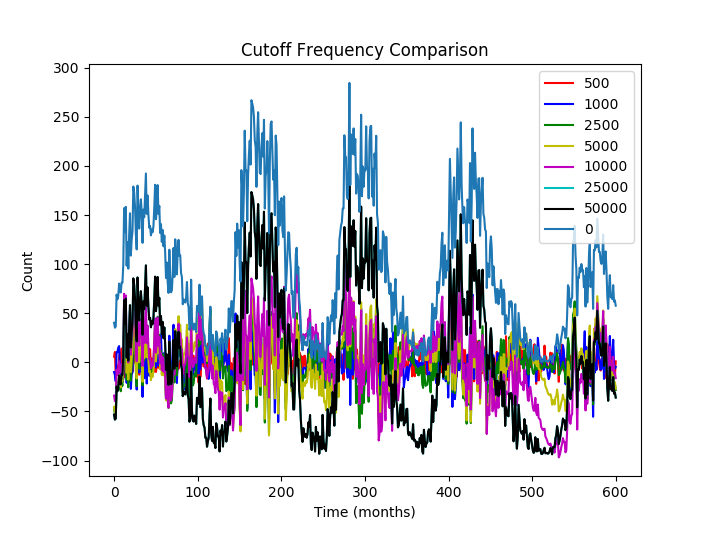
\includegraphics[scale=0.8]{ugly.png}
\end{center}
\end{figure}


Okay, well that wasn't very useful. Here try this instead:

\begin{figure}[H]
\begin{center}
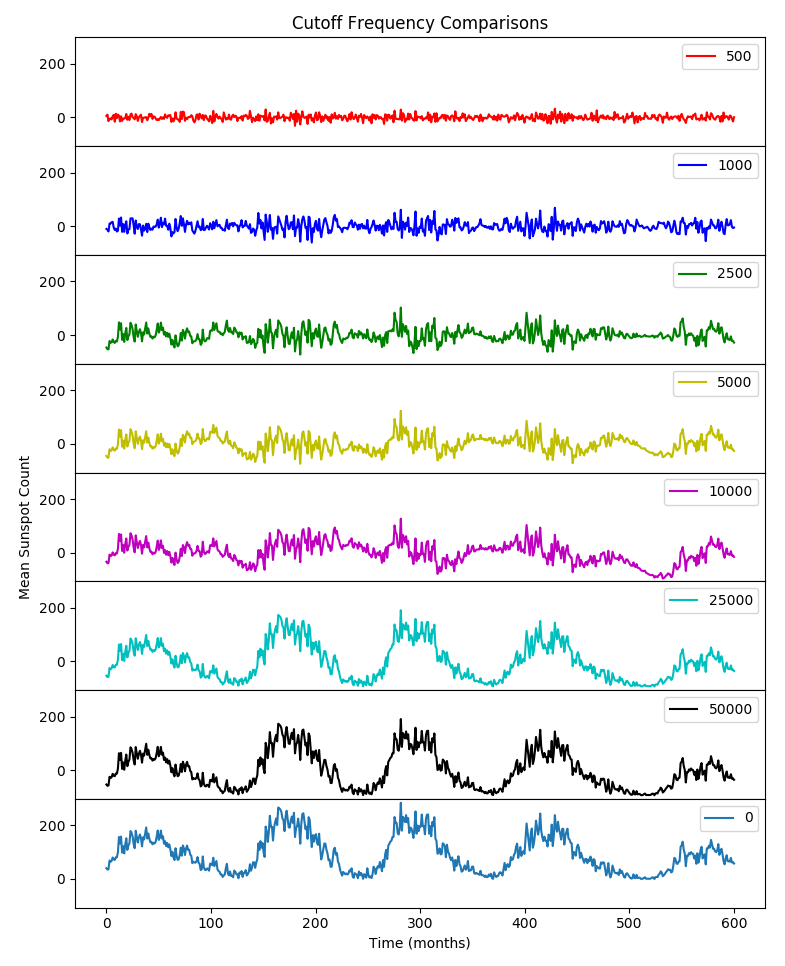
\includegraphics[scale=0.8]{freqs.png}
\end{center}
\end{figure}

Ah, okay, in this plot, we can see the different cutoff frequencies, in ascending order. We can see that we cutoff most data in the first plot, including the data we didn't want to discard. However, near the higher cutoff frequencies, we get basically the original data. The last plot is the original data plotted, ignore the $0$ in the legend. Here is the same plot, but for cosmic rays data instead:

\begin{figure}[H]
\begin{center}
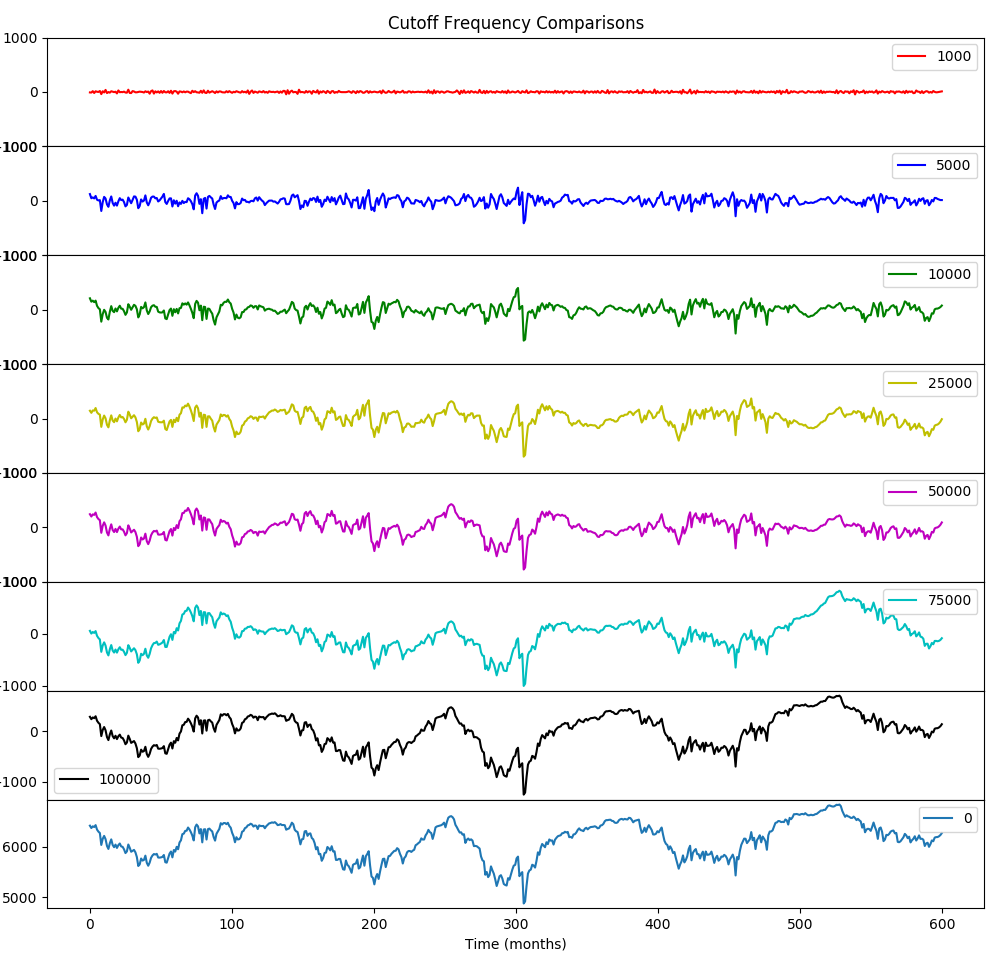
\includegraphics[scale=0.7]{rays_freqs.png}
\end{center}
\end{figure}

I had to use different cutoff frequencies, as it is different data. We can still see the change as the cutoff frequency increases or decreases. The y-axis is the corrected counts/minute of cosmic rays. Again, just like the last plot, the last graph is the original data.

I'm not entirely convinced this helps our data particularly, but it could be because I didn't find the perfect cutoff frequency for our data. Though I did see some improvement, I'm not sure if I would go out of my way to do this, had I done this project again. This may be more useful for a computer application, to filter our unneeded data; however, to my untrained eye, it doesn't seem to help my manual analysis too much.




\section*{Conclusions}

This project was a really great learning experience. Using real world data to come to real conclusions really solidified my understanding of the methods -- it also felt like I was doing real science, instead of just learning theories in usual lectures. My understanding of the Fourier transform was also always a little be foggy, but I learned a lot about it. It was really useful to learn about the Fast Fourier Transform, because in my research online, I learned a lot about how many, many professions, such as audio engineers or astrologists (and physicists, of course!) use the FFT constantly. I'm currently in a acoustics lab that uses the FFT constantly, but to me, it seemed like magic. Now, I understand why it works, and how to manipulate and use it for other purposes, such as signal processing.

I'm excited to try to think of other ways I can use the FFT in my personal projects. Maybe instead of filtering signals, I can map them to other values to change the tone or pitch -- sort of like a voice changer. Maybe that'll be a summer project.




\begin{thebibliography}{9}

\bibitem{a} Josh Samani
\\\texttt{Project 4 PDF}

\bibitem{a} NumPy FFT Docs
\\\texttt{https://docs.scipy.org/doc/numpy-1.12.0/reference/routines.fft.html}

\bibitem{a} NumPy correlate Docs
\\\texttt{https://docs.scipy.org/doc/numpy-1.12.0/reference/generated/numpy.correlate.html}

\bibitem{a} Digital Signal Processing Stack Exchange
\\\texttt{https://dsp.stackexchange.com/questions/736/how-do-i-implement-cross-correlation
-to-prove-two-audio-files-are-similar/739\#739}

\bibitem{a} Python Stack Overflow
\\\texttt{https://stackoverflow.com/questions/643699/how-can-i-use-numpy-correlate
-to-do-autocorrelation}





\end{thebibliography}

\end{document}
